\documentclass{llncs}
\usepackage{graphicx}
\usepackage{amsmath,amssymb} % define this before the line numbering.
\usepackage[mathx]{mathabx}
\usepackage{ruler}
\usepackage{color}
\usepackage{comment}
\usepackage{enumerate}
\usepackage{hyperref}
\usepackage{subcaption}
\usepackage[width=122mm,left=12mm,paperwidth=146mm,height=193mm,top=12mm,paperheight=217mm]{geometry}
\usepackage{booktabs}

\newcommand{\todo}[1]{\textcolor{red}{\textbf{#1}}}
\newcommand{\ECCV}{}
\DeclareMathOperator{\elu}{elu}

\begin{document}
% \renewcommand\thelinenumber{\color[rgb]{0.2,0.5,0.8}\normalfont\sffamily\scriptsize\arabic{linenumber}\color[rgb]{0,0,0}}
% \renewcommand\makeLineNumber {\hss\thelinenumber\ \hspace{6mm} \rlap{\hskip\textwidth\ \hspace{6.5mm}\thelinenumber}}
% \linenumbers
\pagestyle{headings}
\mainmatter

\title{Deep Learning Project Report} % Replace with your title

\titlerunning{Deep Learning Project Report}

\authorrunning{Deep Learning Project Report}

\author{David Flores \and Kirby Linvill}
\institute{CU Boulder}


\maketitle

\begin{abstract}
    % one paragraph summary of your paper describing the motivation, problem, conducted experiments, and experimental findings
    Many state-of-the-art neural networks have been shown to be vulnerable to attacks and adversarial inputs.
    One solution to this problem is to formally verify that a network is robust against classes of attacks.
    Unfortunately, the current state-of-the-art neural network verifiers restrict the network architecture to only use the ReLU, sigmoid, and tanh activation functions.
    We tackle this shortcoming by extending the ETH Robustness Analyzer for Neural Networks (ERAN) to support the ELU activation function.
    We then demonstrate that the extended ERAN performs comparably on networks using the ELU activation function as on networks using only the previously supported activation functions.

    \keywords{Verification, Neural Networks, Robustness, Abstract Interpretation}
\end{abstract}

\section{Introduction}

%paragraph 1: Explain the motivation for your work; e.g., Why anyone should care? What are the desired benefits?
Common neural networks have been shown to be vulnerable to adversarial attacks \cite{szegedy2013intriguing,goodfellow2014explaining,kurakin2016adversarial,carlini2017towards,athalye2018synthesizing,eykholt2018robust,papernot2017practical,papernot2016transferability}.
Adding even slight perturbations to an input that are undetectable by humans can cause a trained neural network to output wildly different results.
Unfortunately, exhaustively testing for perturbations which give divergent results is impractical, especially given large input spaces when using images.
This is where verification methods for neural networks come in, as these techniques allow us to specify constraints and test whether a network meets those constraints (e.g. guarantees that perturbed inputs predict the same output).
There are different approaches to verification, but we focus on the incomplete verification of neural networks.
The incomplete approach to verification gives up completeness, meaning that some constraints that actually do hold may not be verifiable and result in a false positive when attempting to verify the network.
In exchange, these incomplete approaches to verification scale much better to larger networks than complete verification approaches.

%Paragraph 2: Explain why existing solutions work is inadequate for the motivated problem; e.g., Is there a gap in the literature? Is there a weakness in existing approaches?
While existing techniques for verification of neural networks exist, they have only been developed for the most common activation functions, such as the ReLU, tanh, and sigmoid activation functions; yet, many networks use other activation functions as well.
For instance, the LXMERT network \cite{LXMERT} uses GELU activations when performing question answering tasks.
Without testing on neural networks that use these different functions, it is uncertain whether existing techniques are applicable or scale well to these networks.
Thus, it is not known if existing techniques for incomplete verification of neural networks apply to all networks regardless of activation function.

%Paragraph 3: Explain what you are proposing, what is novel/new about your idea, and why you believe this solution will be better than previous solutions; e.g., Are you asking a new question, offering a greater understanding of a research problem, establishing a new methodology to solve a problem, building a new software tool, or offering greater understanding about existing methods/tools?
We extend the existing implementation of some of these verification techniques to  handle activation functions not yet examined in the verification literature.
In particular, we extend the ETH Robustness Analyzer for Neural Networks (ERAN) \cite{ERAN} with an implementation for the ELU activation function.
This requires first formulating relaxations for the ELU function before implementing those relaxations in the ERAN framework.
We then test the implementation following the approaches in \cite{muller2022prima} and \cite{singh2019abstract} to ensure that ERAN with our extensions can verify networks that use ELU functions.
We further test our implementation to see how precise our robustness guarantees are compared to guarantees for an equivalent network when using ReLU, sigmoid, and tanh activation functions instead.
These tests allow us to understand how well these existing techniques for incomplete verification of neural networks apply to new activation functions, and if it is practical to use this technique on realistic networks utilizing ELU.



\section{Related Work}

Many previous research works provide formal robustness guarantees for neural networks.
These works fall into two categories: those that use complete verification approaches and those that use incomplete verification approaches.
Both sets of approaches guarantee soundness, that is they prevent false negatives.
Complete approaches also guarantee completeness, that is they also prevent false positives.
Incomplete approaches give up on completeness in exchange for better scalability.

\subsection{Complete Verification of Neural Networks}
A common approach to complete verification is to frame network robustness in terms of logical constraints that can then be checked using SMT solvers \cite{ehlers2017formal}, \cite{huang2017safety}, \cite{katz2017reluplex}, \cite{katz2019marabou}, \cite{pulina2010abstraction}.
Another common approach leverages branch-and-bound techniques and Mixed Integer and Linear Programming (MILP) solvers \cite{anderson2020strong}, \cite{botoeva2020efficient}, \cite{bunel2020branch}, \cite{lu2019neural}, \cite{de2021scaling}, \cite{tjeng2017evaluating}, \cite{wang2021beta}, \cite{xu2020fast}, \cite{cheng2017maximum}, \cite{fischetti2018deep}, \cite{bunel2018unified}, \cite{dutta2018output}.
Both of these approaches rely on solving NP-complete problems.
As a result, they have trouble scaling to neural networks used today.

\subsection{Incomplete Verification of Neural Networks}
Incomplete verification approaches utilize relaxations and approximations to produce more efficient, albeit less precise, robustness guarantees.
Many previous works use abstract interpretation, a common approach in program analysis, to verify robustness in a particular domain \cite{gehr2018ai2}, \cite{singh2018fast}, \cite{singh2019abstract}, \cite{li2019analyzing}, \cite{urban2020perfectly}, \cite{muller2021scaling}, \cite{muller2022prima}, \cite{zhang2020verification}, \cite{mirman2018differentiable}, \cite{muller2020neural}, \cite{singh2019beyond}.
For example, the interval domain is used to abstract out real-valued variables so that each variable is replaced with the bounds on the values it can take (e.g. $\{[a,b] \; | \; a,b \in \mathbb{R} \cup \{-\infty, \infty\}\}$).
Many other works instead use linear approximations to make bounds computations more efficient \cite{weng2018towards}, \cite{singh2018boosting}, \cite{zhang2018efficient}, \cite{balunovic2019certifying}, \cite{ruoss2020efficient}, \cite{ko2019popqorn}, \cite{gowal2019scalable}, \cite{bunel2020efficient}, \cite{lyu2020fastened}, \cite{tjandraatmadja2020convex}.
Others rely on using techniques from simulation \cite{xiang2018output}, duality \cite{wong2018provable}, \cite{dvijotham2018dual}, and semidefinite programming \cite{raghunathan2018certified}, \cite{dathathri2020enabling}, \cite{raghunathan2018semidefinite}.
Another strain of works look instead at probabilistic robustness guarantees rather than deterministic ones using randomized smoothing \cite{cohen2019certified}, \cite{lecuyer2019certified}, \cite{salman2019provably}.

Though these works on both complete and incomplete approaches have shown impressive results formally verifying the robustness of neural networks, they only implement and evaluate ReLU, sigmoid, and tanh activation functions.
As a result, these works cannot verify common networks including the LXMERT network with a question answering head that uses GELU \cite{GELU} activations.
To move towards supporting verification of these networks, we extend the ETH Robustness Analyzer for Neural Networks (ERAN) \cite{ERAN} to support the common ELU \cite{ELU} activation functions.
ERAN is a state-of-the-art verification tool based on abstract interpretation and the work done in \cite{singh2018fast}, \cite{singh2019abstract}, \cite{singh2018boosting}, \cite{singh2019beyond}, \cite{balunovic2019certifying}, \cite{ruoss2020efficient}, \cite{muller2021scaling}, and \cite{muller2022prima}.
To the best of our knowledge, our work is the first time neural networks with these activation functions have been supported by formal robustness analyses.



\section{Methods}
ERAN relies on the ETH Library for Numerical Analysis (ELINA) \cite{ELINA} to implement support for numerical abstract domains.
In particular, ELINA includes the code responsible for handling the relaxations for each layer in a neural network including activation layers.
As a result, we supply our own relaxations for the ELU activation function as extensions of DeepPoly \cite{singh2019abstract} within ERAN.
This requires providing sound upper and lower bounds along with upper and lower polyhedral constraints of the activation functions' outputs as a function of their input values.
The polyhedral constraints for variable $x_i$ have the form $v + \sum_j w_j \cdot x_j$ where $v \in \mathbb{R} \cup \{-\infty, \infty\}$, $w \in \mathbb{R}^n$, $\forall j \geq i. \; w_j = 0$.
Node outputs are represented by variables $x_i$ that are uniquely numbered such that any node that receives inputs from other nodes must be given a greater number than their inputs.
As a result, constraints for variables $x_i$ can refer to earlier variables in the network but not later variables since for all  $j \geq i$, $w_j = 0$.

We adapt the existing implementations of the sigmoid and tanh bounds and constraints to implement ELU bounds and constraints.
The sigmoid and tanh constraints rely on a generic transformation that requires the activation function $g: \mathbb{R} \rightarrow \mathbb{R}$ to be twice differentiable and satisfy $g'(x) > 0$ and $0 \leq g''(x) \Leftrightarrow x \leq 0$.
ELU meets this requirement so we can directly adapt the constraints and bounds from sigmoid and tanh.
In particular, this means we set the lower and upper bounds for ELU as $l_j = \elu({l_i})$ and $u_j = \elu({u_i})$ where $l_i$ and $u_i$ are the input lower and upper bounds respectively.
It also means we set the polyhedral constraints as follows.
Let $\lambda$ be the slope of the line between $\elu(l_i)$ and $\elu(u_i)$.
That is, $\lambda = (\elu(u_i) - \elu(l_i)) / (u_i - l_i)$.
If we are solely in the linear region, that is $l_i \geq 0$, then we set the lower constraint to $\elu(l_i) + \lambda \cdot (x_i - l_i)$.
Otherwise, we set the lower constraint to $\elu(l_i) + \min(\elu'(l_i), \elu'(u_i)) \cdot (x_i - l_i)$.
If we are solely in the exponential region, that is $u_i \leq 0$, then we set the upper constraint to $\elu(u_i) + \lambda \cdot (x_i - u_i)$.
Otherwise, we set the upper constraint to $\elu(u_i) + \min(\elu'(l_i), \elu'(u_i)) \cdot (x_i - u_i)$.
As shown in Fig. \ref{fig:elu_relax}, these approximations are tight in the exponential region (\ref{fig:elu_exp_relax}) and exact in linear region (\ref{fig:elu_linear_relax}).
However, the approximations are loose when the lower and upper bounds span both the linear and exponential regions (\ref{fig:elu_mixed_relax}).
% TODO(klinvill): Do we want to spell out a tighter approximation here and just not implement it? In particular, since ELU is convex, we can just always use a line between ELU(l_i) and ELU(u_i) as the upper bound.
A tighter approximation is left for future work.

\begin{figure}[t]
    \centering
    \begin{subfigure}{.48\textwidth}
        \centering
        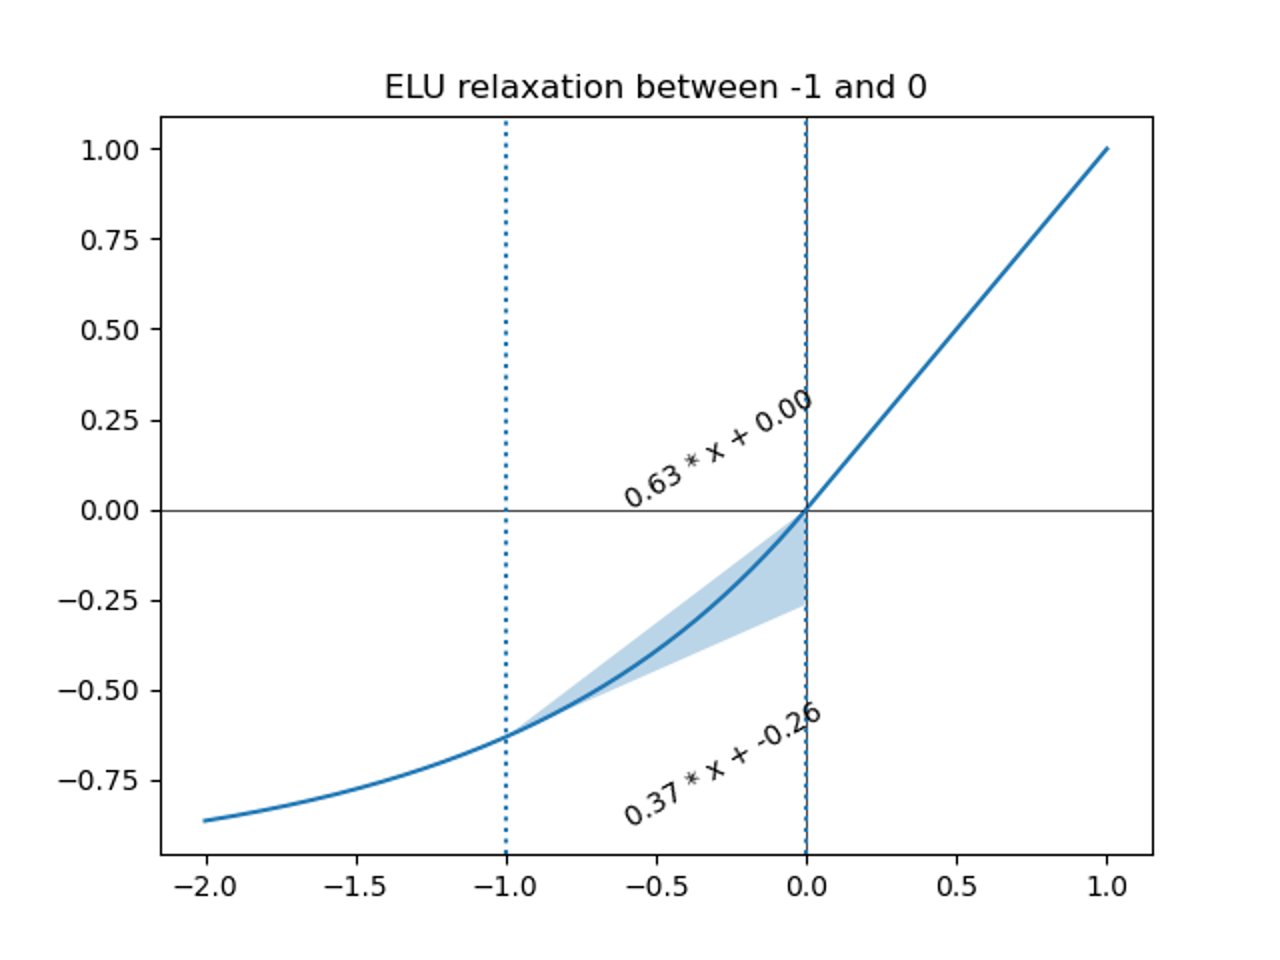
\includegraphics[width=\linewidth]{elu_exponential_relaxation.png}
        \caption{Our approximation is tight in the exponential region of ELU.}
        \label{fig:elu_exp_relax}
    \end{subfigure}
    \quad
    \begin{subfigure}{.48\textwidth}
        \centering
        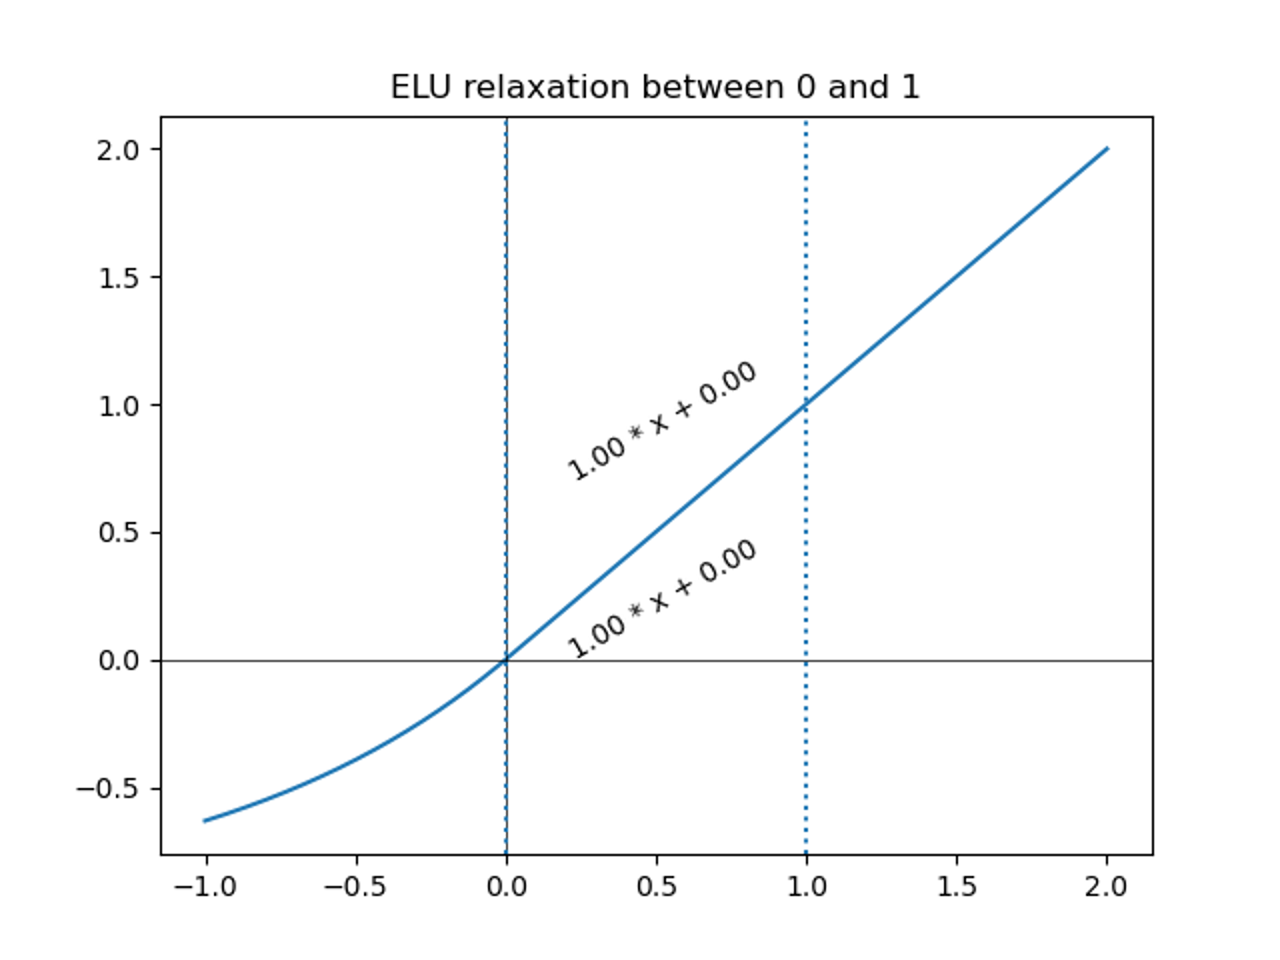
\includegraphics[width=\linewidth]{elu_linear_relaxation.png}
        \caption{And our approximation is exact in the linear region of ELU.}
        \label{fig:elu_linear_relax}
    \end{subfigure}
    \begin{subfigure}{.48\textwidth}
        \centering
        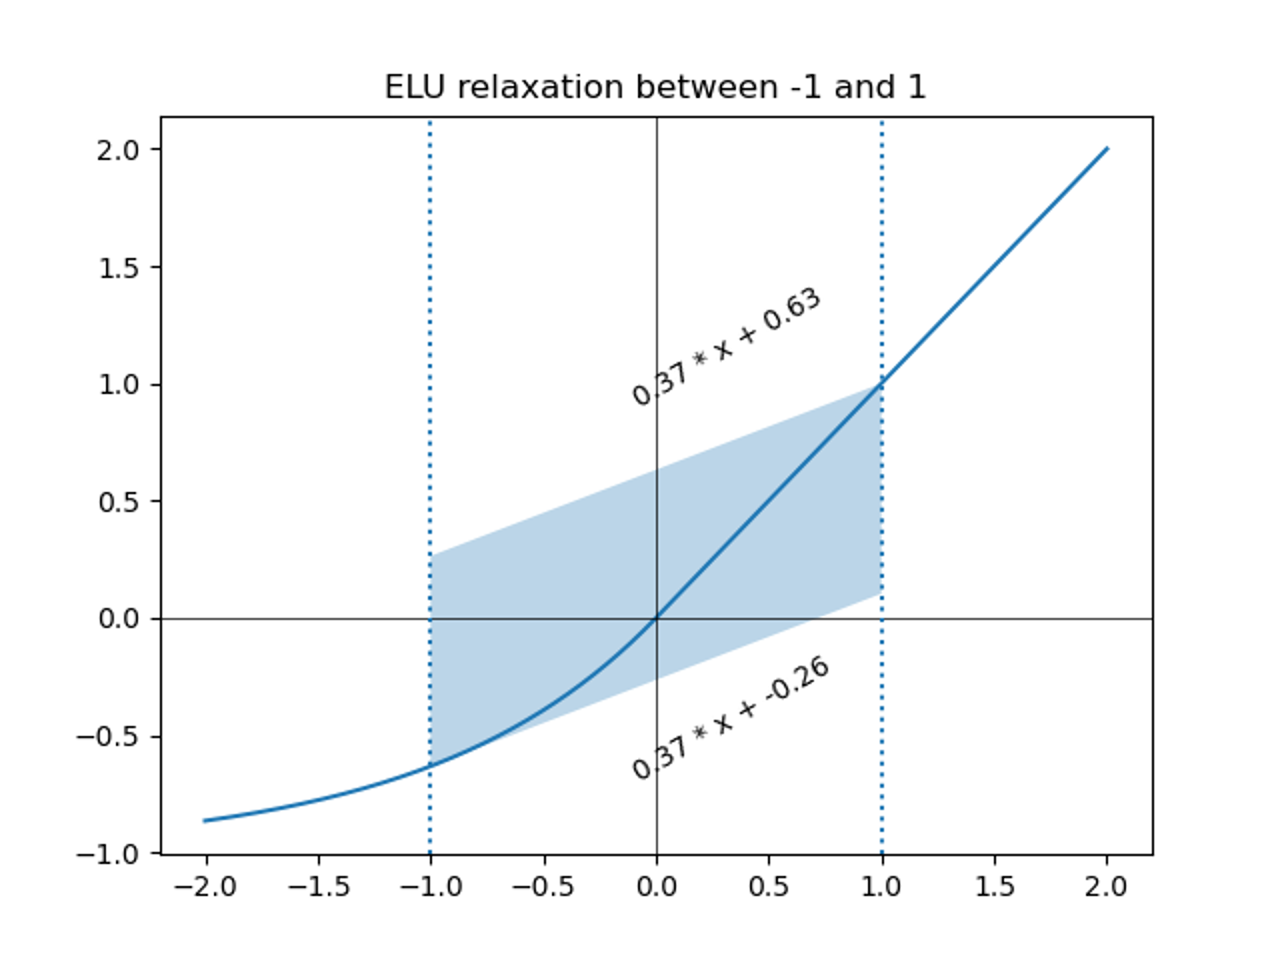
\includegraphics[width=\linewidth]{elu_mixed_relaxation.png}
        \caption{Yet our approximation is loose when spanning both the linear and exponential regions of ELU.}
        \label{fig:elu_mixed_relax}
    \end{subfigure}
    \caption{ELU Relaxation}
    \label{fig:elu_relax}
\end{figure}

\section{Soundness of ELU Relaxation}
To ensure our relaxations are sound, we need to show that they over-approximate the output space.
We can show soundness by showing that any output from the activation function is contained between the predicted lower and upper constraints and that the abstract relaxations over-approximate the concrete relaxations.
For DeepPoly, the first property is formalized as $\gamma_i(a') \subseteq \bigtimes_{k\in[i]}[l_k',u_k']$ where $a'$ is any relaxed output of the activation function (in its abstracted form) and $\gamma$ is the concretization function for the abstract domain.
The second property is formalized as $T_f(\gamma_{i-1}(a)) \subseteq \gamma_i(a')$ where $a$ is the abstract relaxed input of activation function and $T_f$ is a concrete transformer that implements the relaxation.

The general relaxation for sigmoid and tanh is shown to be sound in \cite{singh2019abstract}.
We claim our ELU approximation is sound by the same proof since we adapt the same scheme.
However, we provide a sketch of soundness in the concrete domain for the reader.
We show overall soundness by showing soundness for three cases: when the relaxation is solely in the linear region of ELU ($x \geq 0$), when the relaxation is solely in the exponential region of ELU ($x \leq 0$), and when the relaxation covers both regions.

Across all three cases we let $g_u(x)$ represent the upper constraint and $g_l(x)$ represent the lower constraint for our relaxation.
To show soundness, we simply need to show that for all $l_i \leq x \leq u_i$ both $g_u(x) \geq \elu(x)$ and $g_l(x) \leq \elu(x)$.

\subsection{Soundness in the Exponential Region}
We first consider the upper constraint $g_u(x)$.
In the exponential region, $g_u(x) = \elu(u_i) + \lambda \cdot (x - u_i)$ where $\lambda = (\elu(u_i) - \elu(l_i)) / (u_i - l_i)$.
Consequently $g_u(u_i) = \elu(u_i)$ and $g_u(l_i) = \elu(l_i)$.
Since both $\elu'(x) > 0$ and $g_u'(x) > 0$, that is, $\elu$ and $g_u$ are both monotonically increasing, we can conclude that $\max(g_u(x)) = g_u(u_i) = \elu(u_i) = \max(\elu(x))$ and $\min(g_u(x)) = g_u(l_i) = \elu(l_i) = \min(\elu(x))$ within the bounds $l_i \leq x \leq u_i$.
We can also see that $\elu''(x) > 0$ in this region meaning that the function is convex.

Since $\elu$ is convex, we know that $s\elu(l_i) + (1-s)\elu(u_i) \geq \elu(s\cdot l_i + (1-s)\cdot u_i)$ for all $s\in [0, 1]$.
Furthermore, since $g_u$ is linear, it follows that $s g_u(l_i) + (1-s) g_u(u_i) = g_u(s\cdot l_i + (1-s)\cdot u_i)$
For all $l_i \leq x \leq u_i$, there exists $s\in[0,1]$ such that $x = s\cdot l_i + (1-s)\cdot u_i$.
So, we see that
\begin{align*} 
    g_u(x) &= g_u(s\cdot l_i + (1-s)\cdot u_i) \\
           &= s g_u(l_i) + (1-s) g_u(u_i) \\
           &= s \elu(l_i) + (1-s) \elu(u_i) \\
           &\geq \elu(s\cdot l_i + (1-s)\cdot u_i) \\
           &= \elu(x).
\end{align*}
Thus we have $g_u(x) \geq \elu(x)$, which meets our definition of soundness for the upper constraint.

Similarly, the lower constraint in the exponential region is $g_l(x) = \elu(l_i) + \min(\elu'(l_i), \elu'(u_i)) \cdot (x - l_i) = \elu(l_i) + \elu'(l_i) \cdot (x - l_i)$.
Consequently $g_l(l_i) = \elu(l_i)$.
Since $\elu'(x) \geq 0$ and $g_l'(x) \geq 0$, that is, $\elu$ and $g_l$ are both monotonically increasing, we can conclude that $\min(g_l(x)) = g_l(l_i)$ and $\elu(l_i) = \min(\elu(x))$ which means that $\min(g_l(x)) = \min(\elu(x))$.
Additionally, because $\elu''(x) \geq 0$, such that $\elu'$ is monotonically increasing, we know that $\min(\elu'(x)) = \elu'(l_i)$ and that $g_l'(x) \leq \elu'(x)$ when $l_i \leq x$.
Since $\min(g_l(x)) = \min(\elu(x))$ and $g_l'(x) \leq \elu'(x)$,
we see that 
$$ \frac{d}{dx}\left( \elu(x) - g_l(x) \right) = \elu'(x) - g_l'(x) \geq 0, $$
and $\elu(l_i) -g_l(l_i) \ge 0$.
Thus, we see that for $l_i \leq x \leq u_i$, $\elu(x) - g_l(x)$ is monotonically increasing, with minimum value $\elu(l_i) - g_l(l_i) = 0$, and hence $\elu(x) - g_l(x) \geq 0$.
This can be rearranged to $\elu(x) \geq g_l(x)$, which meets our definition of soundness for the lower constraint.
% we can therefore reason that $g_l(x) \leq \elu(x)$ for $l_i \leq x$.
% This meets our definition of soundness for the lower constraint.

Our relaxation is therefore sound in the exponential region since both the upper and lower constraints are sound.

\subsection{Soundness in the Linear Region}
We again first consider the upper constraint $g_u(x)$.
In this region, we recall that $g_u(x) = \elu(u_i) + \min(\elu'(l_i), \elu'(u_i))\cdot (x-u_i)$, which we can simplify to
$g_u(x) = u_i + 1 \cdot (x-u_i) = x$ as $\elu(x)=x$ and hence $\elu'(l_i)=\elu'(u_i)=1$ in the linear region.
Hence, we see that $g_u(x) = \elu(x)$.
This is both an exact and sound approximation.

Similarly for the lower constraint it is the case that
$\lambda = (\elu(u_i) - \elu(l_i))/(u_i - l_i) = (u_i - l_i)/(u_i - l_i) = 1$, and hence
$g_l(x) = \elu(l_i) + \lambda \cdot (x - l_i) = l_i + (x - l_i) = x$.
So, $g_l(x) = \elu(x)$ and the lower constraint is both an exact and sound approximation.

Our relaxation is therefore both sound and exact in the linear region since both the upper and lower constraints are both sound and exact.

\subsection{Soundness When Spanning Both Regions}
We again first consider the upper constraint $g_u(x)$.
In this case, $g_u(x) = \elu(u_i) + \min(\elu'(l_i), \elu'(u_i)) \cdot (x - u_i) = \elu(u_i) + \elu'(l_i) \cdot (x - u_i)$.
Consequently $g_u(u_i) = \elu(u_i)$.
Since $\elu'(x) \geq 0$ and $g_u'(x) \geq 0$, such that $\elu$ and $g_u$ are monotonically increasing, we conclude that $\max(g_u(x)) = g_u(u_i)$ and $\elu(u_i) = \max(\elu(x))$ which means that $\max(g_u(x)) = \max(\elu(x))$ when $x \leq u_i$.
Additionally, because $\elu''(x) \geq 0$, such that $\elu'$ is monotonically increasing, we know $\min(\elu'(x)) = \elu'(l_i)$ and hence $\elu'(x) \geq g_u'(x)$ when $x \geq l_i$.
Since $\max(g_u(x)) = \max(\elu(x))$ and $\elu'(x) \geq g_u'(x)$,
we see that 
$$ \frac{d}{dx}\left( g_u(x) - \elu(x) \right) = g_u'(x) - \elu'(x) \geq 0, $$
and $g_u(l_i) - \elu(l_i) \ge 0$.
Thus, we see that for $l_i \leq x \leq u_i$, $g_u(x) - \elu(x)$ is monotonically increasing, with minimum value $g_u(l_i) - \elu(l_i) = 0$, and hence $g_u(x) - \elu(x) \geq 0$.
This can be rearranged to $\elu(x) \leq g_u(x)$, which meets our definition of soundness for the upper constraint.
% we can therefore reason that $g_u(x) \geq \elu(x)$ for $l_i \leq x \leq u_i$.
% The upper constraint is therefore a sound upper constraint when spanning both the linear and exponential regions.

The proof of soundness for the lower constraint in this case is identical to the proof of soundness for the lower constraint in the exponential region. We can therefore conclude our relaxation is sound when spanning both the linear and exponential regions since both the upper and lower constraints are sound.


\section{Experimental Design}
% Describe 1-2 experiments or analyses you plan to conduct in order to demonstrate/validate the target contribution(s) of your work. Your description should be detailed enough so that a reader could reproduce it. Your description should include the following for each experiment:
% \begin{itemize}
%     \item Main purpose: 1-3 sentence high level explanation
%     \item Evaluation Metric(s): which ones will you use and why?
% \end{itemize}

To validate and evaluate our ELU relaxation and implementation, we trained and verified models using the ELU activation function against the MNIST dataset and compared the results to models using the ReLU, sigmoid, and tanh activation functions.
We used the same model architecture for all models, only varying the activation functions.
The models have 5 fully connected hidden layers with 100 neurons per layer.
We trained the models in DiffAI \cite{mirman2018differentiable} using two different approaches: one using ordinary training techniques (the Point domain in DiffAI) and one using a defensive training technique (a mix of the Projected Gradient Descent \cite{madry2017towards}, or PGD, and the BiAdv domain using Iterated Fast Gradient Sign Method \cite{goodfellow2014explaining}, or IFGSM).
Specifically we used the domain recommended by DiffAI: 
\begin{verbatim}
    Mix(a=PGD(r=3,k=16,restart=2, w=0.1),
        b=BiAdv(a=IFGSM(k=5, w=0.05)), bw=0.1)
\end{verbatim}
The models were all trained for 10 epochs using the MNIST dataset in DiffAI.
All input images were scaled so that pixel values were in the range $[0,1]$.

Once the models were trained, we tested each model using ERAN on a series of verification trials.
The verification challenges we tested included $L_\infty$-norm perturbations \cite{carlini2017towards} of various sizes, with $0.005 \leq \epsilon \leq 0.1$ and centers drawn from ERAN's test set of 100 MNIST images.
The $L_\infty$-norm perturbations randomly adjust each pixel value by up to $\pm \epsilon$.
Since our pixel values and $\epsilon$ values are in the range $[0,1]$, $\epsilon$ can also be seen as a percentage of a maximum possible pixel value.
In addition to testing against ERAN's test set, we also tested against the MNIST test dataset in DiffAI.
We gathered accuracy metrics for both test sets, as well as the number of correctly predicted images that were robust for perturbations up to $\epsilon$.
Accuracy was a reasonable metric given that our test datasets were well balanced.

The code we used to do the training is available on github at \url{https://github.com/DeepLearningVerificationProject}. All training and evaluation was done using the following commits:
\begin{verbatim}
    DiffAI: c60d5bfdfece42bb66347ed6e5120e634ac9ccd3
    ERAN:   3ce9d0adfe789dbef30406c60f6c321d9c7df9ac
    ELINA:  e1b1d463b20b4d096e26fb464d0516f99837b7be
\end{verbatim}

\section{Experimental Results}
%This should include the raw results, what general trends are observed, and insights/speculations into why your results may be turning out the way they are.

%Also include at least one paragraph explaining what questions are not fully answered by your experiments and natural next steps for this direction of research.


As shown in Fig. \ref{fig:verified_pct}, we were able to verify the ELU models for small values of epsilon for all images that were correctly classified. This shows that our extension functionally works.
However, there were several notable trends that emerged from our results.

\begin{figure}[h]
    \centering
    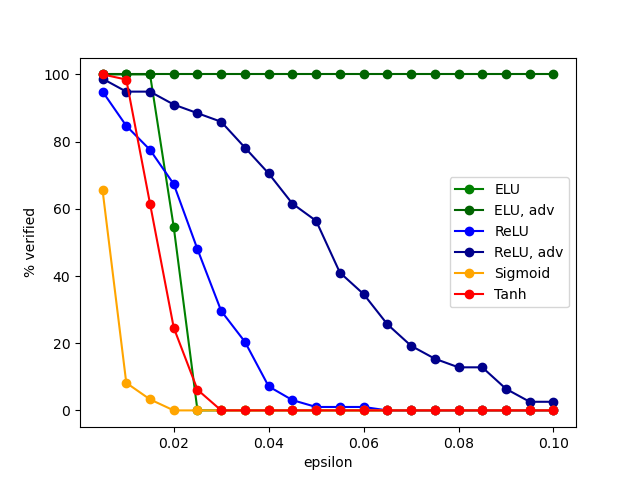
\includegraphics[width=\linewidth]{verified_pct_plot.png}
    \caption{Percentage of correct predictions verified to be robust. The adv models were trained using defensive techniques to increase model robustness.}
    \label{fig:verified_pct}
\end{figure}

As expected, the number of correct predictions that could be verified to be robust against $L_\infty$-norm perturbations with given $\epsilon$ decreased as $\epsilon$ increased.
$\epsilon$ represents the magnitude of the perturbations in the range [0, 1] such that
$\epsilon = 0$ corresponds to no perturbation while $\epsilon = 1$ corresponds to perturbations that can push any pixel to any value between its min and max ([0, 255] in the MNIST dataset).
Unsurprisingly, very few predictions could be verified to be robust at $\epsilon = 0.1$.
It is also unsurprising that networks that were trained without defensive techniques were much less robust than their defensively trained counterparts.

However, it is surprising that the defensively trained ELU network could verify all predictions to be robust up to large values of $\epsilon$, including $\epsilon = 1$.
Coupled with the fact that the defensively trained ELU network could only correctly predict $\sim 10\%$ of the ERAN test images as shown in Table \ref{tab:model_accuracies}, these facts imply that the model predicts the same label regardless of the input.
Indeed upon further inspection the model always predicted the label 3 when run in ERAN, yet was $98\%$ accurate when manually tested against the images ERAN uses as its test set.
When ERAN runs a model against the test set, it does not use the concrete model for predictions but rather the abstract model that utilizes the relaxations for the activation functions.
From the set of possible output labels, it then chooses the first label as the prediction.
So, if the abstract model is imprecise enough, ERAN will always predict the same label for the model regardless of the input.
It is interesting that only the defensively trained ELU model predicts the same label without fail, but this phenomena is likely explained by the fact that our relaxation of ELU is tight in the exponential region and exact in the linear region, so the normally trained ELU model may simply be using ELU more frequently in either the exponential or linear regions.

\begin{table}[h]
    \centering
    \caption{Model performance on the test set ($n=2000$) and on ERAN's test set ($n=100$).}
    \bigskip
    \begin{tabular*}{\linewidth}{@{\extracolsep{\fill}}llll@{}}
        \toprule
        activation function & defensively trained & test accuracy & ERAN test accuracy \\
        \midrule
        ELU     & no    & 0.98 & 0.11 \\
        ELU     & yes   & 0.94 & 0.14 \\
        ReLU    & no    & 0.98 & 0.98 \\
        ReLU    & yes   & 0.87 & 0.78 \\
        Sigmoid & no    & 0.97 & 0.61 \\
        Tanh    & no    & 0.96 & 0.65 \\
        \bottomrule
    \end{tabular*}
    \label{tab:model_accuracies}
\end{table}

We believe the same root cause is behind the fact that the ReLU models performed comparably on the test set and the ERAN's test set while all the other models performed dramatically worse on ERAN's test set.
The ReLU relaxation is exact in both the linear and exponential regions and tight when spanning both regions unlike the sigmoid, tanh, and ELU relaxations.
It is likely that the dramatic drop in performance is primarily due to the abstract model being too over-approximate thereby leading to more incorrect predictions.
The slight drop in performance for the defensively trained ReLU model could be either an artifact of the small size of ERAN's test set or due to the ReLU activations in the model frequently operating across both the linear and exponential regions (thereby leading to a less precise abstract model).
Improved performance on the ERAN test set could likely be achieved by developing tighter approximations of the activation functions.

A natural next step for this work is to conduct a closer examination of the abstract models to validate or disprove our hypothesis about the poor performance on the ERAN test set.
Assuming our hypothesis is correct, it would be very valuable to develop tighter approximations of the activation functions.
Tighter approximations could be achieved by using a different abstract domain, better relaxations, or by moving to multi-neuron approximations instead of the single-neuron approximations we use in this paper.
Further work could also add support for more activation functions including the GELU activation function which is widely used in state-of-the-art transformers.

\section{Conclusions}
%Summarize in one paragraph what is the main take-away point from your work.
In this work, we investigate if current neural network verification work can be extended to include networks using less common activation functions such as the ELU activation function.
To this end, we create and prove sound an approximation of the ELU activation function, and use the approximation to run verification experiments on the networks in question.
This work shows some promise in the extension to the ELU activation function, however our experiments also generated some unexpected results.
For the images for which the ELU model predicted the correct output, a similar percentage of the corresponding constraints were able to be verified as when using other models with already tested activation functions.
Unfortunately, only a small number of images in the verification set were correctly predicted using the ELU model.
Nevertheless, we believe that a more precise approximation of the ELU function may fix the issue.

%Add a final paragraph discussing any potential ethical implications of your project (e.g., fairness, accountability, transparency, privacy, social impact, etc).
This work helps pushes the boundary of what type of networks are verifiable, which is useful for developers looking to show robustness of their networks.
While verifying a network can reduce the attack surface for these networks to be manipulated by bad actors, it does not necessarily provide a guarantee of fairness, or address other potential ethical issues.
It is up to the network designers to ensure the constraints they are verifying are sufficient for the use case of the network.
For example, a network for use in a self driving car should likely be subject to stronger constraints, such as a larger epsilon value for $L_\infty$-norm perturbations, than a image classifier for a creating captions on sites like YouTube.
Similarly, it may be possible to create the proper constraints that can be verified to show some degree of fairness, it is up to the network designers to ensure fairness.

\clearpage

\bibliographystyle{splncs}
\bibliography{project_proposal}
\end{document}
